\chapter{MATLAB Exercises}
\section{Mean estimation on heterogeneous data}
In this exercise, we are going to use Monte Carlo simulations to verify the theoretical results obtained in the exercise \ref{sec:ex_1} and provide an analysis of the estimators $\hat\theta_1$, $\hat\theta_2$, $\hat\theta_{ave}$ and $\hat\theta_{ML}$ with varying parameters.

\subsection*{Variation of $\sigma_2^2$}
\begin{figure}[H]
    \centering
    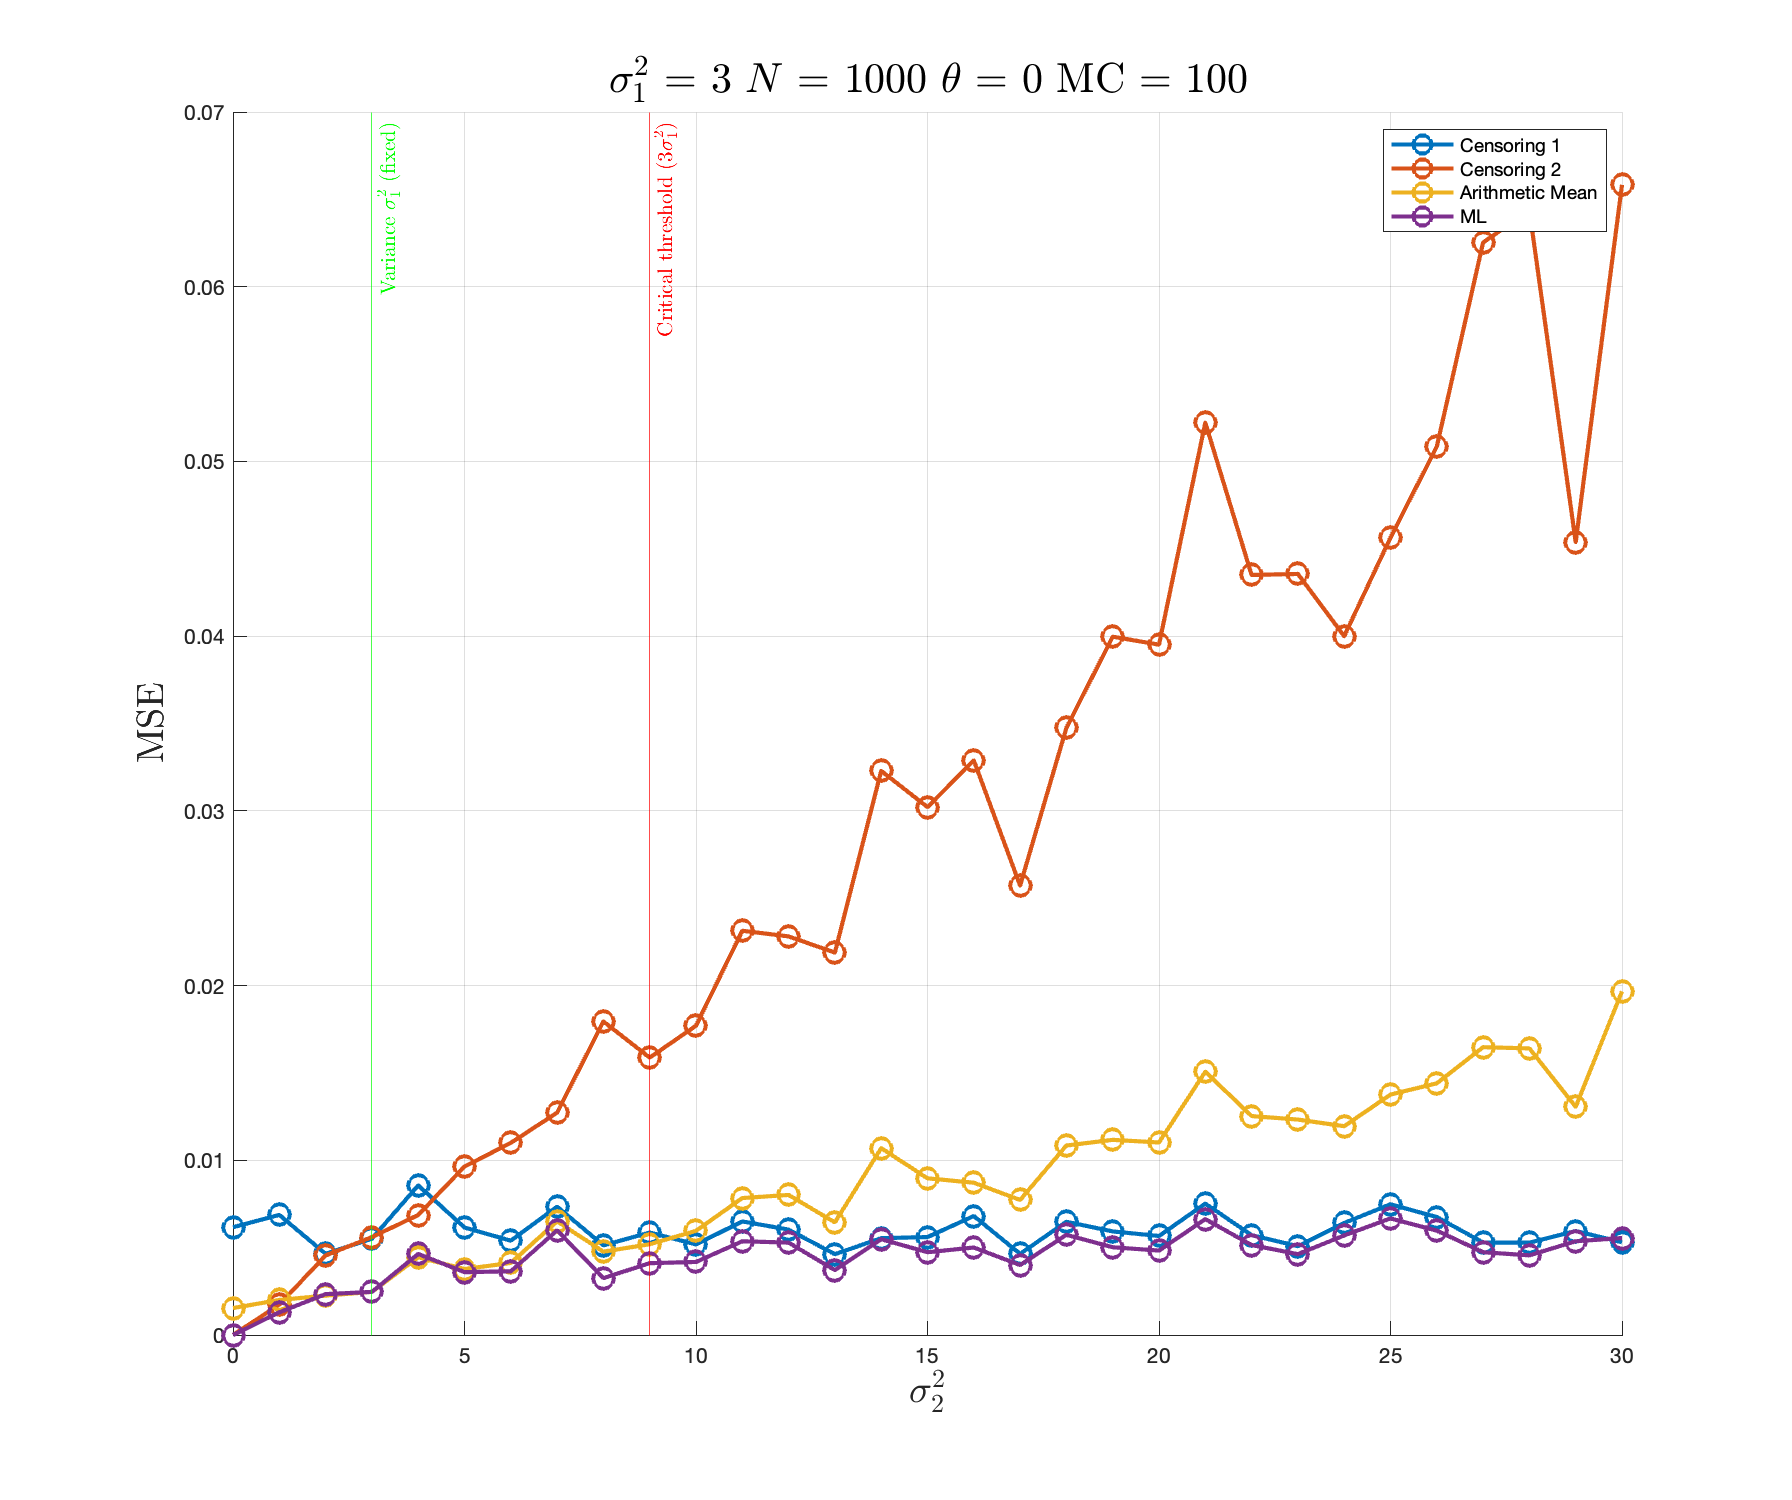
\includegraphics[width=0.8\textwidth]{./figures/appendix_a/figure_1.png}
    \caption{MSE of the estimators $\hat\theta_1$, $\hat\theta_2$, $\hat\theta_{ave}$ and $\hat\theta_{ML}$ as a function of $\sigma_2^2$.}
    \label{fig:mean_estimation_heterogeneous_data}
\end{figure}

Each point is an empirical estimate of the MSE obtained through Monte Carlo simulation, so we will not have exactly the behavior that the theoretical MSE would have, but we are approximating it and this approximation improves by increasing the number of Monte Carlo experiments.

Since we are varying $\sigma_2^2$ we expect the MSE with respect to the estimates made by $\hat \theta _1$ (blue line) to be a constant, remembering however what was said in the first observation to see oscillations is normal being an estimate but increasing $MC$ this approximation can only improve and increasingly resemble a constant.

The MSE shape of $\hat \theta_{ave}$ (yellow line) is increasing as a function of $\sigma^2_2$. It is reasonable since we are adding noise to the system. Since we know the variance of this estimator we also know its theoretical MSE and from it we can observe that the error is linear with respect to $\sigma_2^2$.

From the theoretical analysis we had obtained that there is a special point after which discarding one of the two parts of data is preferable to keeping them equally into account. Therefore, $\hat \theta_{ave}$ (yellow line) which equally weights ($p=0.5$) both parts of data is preferable to $\hat\theta_1$ (blue line) which instead discards completely one part of data (the one that in the graph is increasing its variance) up to this special point which is equal to $3\sigma_1^2$ and represents a level of critical noise for the variance of that slice of data. Beyond this critical point it is preferable to use the estimator $\hat \theta_1$; also from the graph it can be seen how its MSE remains lower than that of $\hat \theta_{ave}$ from the right of the threshold onwards.

It follows that if we wanted to choose between these two the best estimator we would obtain a curve that before the threshold is linear with $\sigma^2_2$ (i.e. $\hat \theta_{ave}$) and after the threshold is a constant, so we would generally have a non-linear behavior as at a certain point there will be a sudden saturation of the error.

The threshold can be read in two different ways depending on whether we vary $\sigma_1^2$ or $\sigma_2^2$.    
\[
\begin{cases}
\sigma_2^2>3\sigma_1^2 \lor \sigma_1^2<\frac 13\sigma_2^2\quad\text{$\hat\theta_1$ better than $\hat \theta_{ave}$}\\
\sigma_2^2<3\sigma_1^2\lor \sigma_1^2>\frac13\sigma_2^2\quad\text{$\hat \theta_{ave}$ better than $\hat \theta_1$ }
\end{cases}
\]
    
\[
    \begin{cases}
    \sigma_1^2>3\sigma_2^2\lor \sigma_2^2<\frac 13\sigma_1^2\quad\text{$\hat\theta_2$ better than $\hat \theta_{ave}$}\\
    \sigma_1^2<3\sigma_2^2\lor \sigma_2^2>\frac13\sigma_1^2\quad\text{$\hat \theta_{ave}$ better than $\hat \theta_2$ }
    \end{cases}
\]

The MSE computed on the estimates made by $\hat \theta_2$ (red line) increases linearly, as we are inserting more and more noise in that slice of data and therefore we are making the estimate more and more difficult at the same $N$.

The estimator $\hat \theta_{ML}$ with respect to all the other estimators is the best over the entire range of variation as the curve of the MSE calculated on its estimates (purple line) always takes lower values. Only at infinity, it seems to converge with the estimator $\hat \theta_1$ and this is what we would expect from the theory.
If we didn't have any formula to support and therefore we should rely only on the data and the simulation we could never be firmly convinced that the MSE of $\hat\theta_{ML}$ is always better than $\hat \theta_1$ as they are too close and it could be just a case that the purple line is lower over the entire range (as experiments we could never be sure). What we could do in a situation like this is:
\begin{enumerate}
    \item Do experiments with different orders of magnitude for the number of Monte Carlo simulations and see if there is a common trend
    \item If at the same data, the curves are very irregular and despite this there is a curve that always has lower values than another, it could be a clue that this phenomenon is also true in theory
\end{enumerate}
When $\sigma_1^2=\sigma_2^2$ the two points of the two curves of the MSE of $\hat\theta_1$ and $\hat\theta_2$ assume the same identical value. The same value for the curves of $\hat\theta_{ML}$ and $\hat\theta_{ave}$ because the weights given by the ML estimator are equal to those implicit in the arithmetic mean ($p=0.5$).
When $\sigma_2^2=0$ we have a slice of data that is giving us exactly the value of the unknown parameter $\theta$, and therefore the MSE of $\hat\theta_2$ will clearly be $0$. In this particular circumstance the performance of $\hat\theta_2$ is equal to that of $\hat\theta_{ML}$.
When $\sigma_2^2\to+\infty$ the ML estimator will tend to give less and less weight to that slice of data as it becomes more and more noisy and therefore asymptotically the performance of $\hat\theta_{ML}$ will be equal to those of $\hat \theta_1$ and in particular will converge to a certain value.

The two previous points show the boundaries of the performance of the ML estimator. In both cases there is a fixed variance, and there is a variance that dominates the other. In one case we have $\sigma_1^2$ fixed and dominated by $\sigma_2^2$, so the slice of data with variance $\sigma_2^2$ becomes "optimal" and the ML estimator moves in that direction. Conversely in the second case $\sigma_1^2$ is still fixed but dominated by $\sigma_2^2$ which in this case indicates that its part of data is becoming worse, so the ML estimator directs its estimates based on the "best" slice of data.

The arithmetic mean cannot guarantee the behavior of the previous point because it does not take into account the parameters so regardless of the value that the variance continues to take information in the same way from both slices of data.

Taking the three estimators $\hat\theta_{ave}$, $\hat\theta_{1}$ and $\hat\theta_{2}$ the curve obtained by properly selecting the best of them at each point is not so different from the curve of $\hat \theta_{ML}$.

\begin{figure}[H]
    \centering
    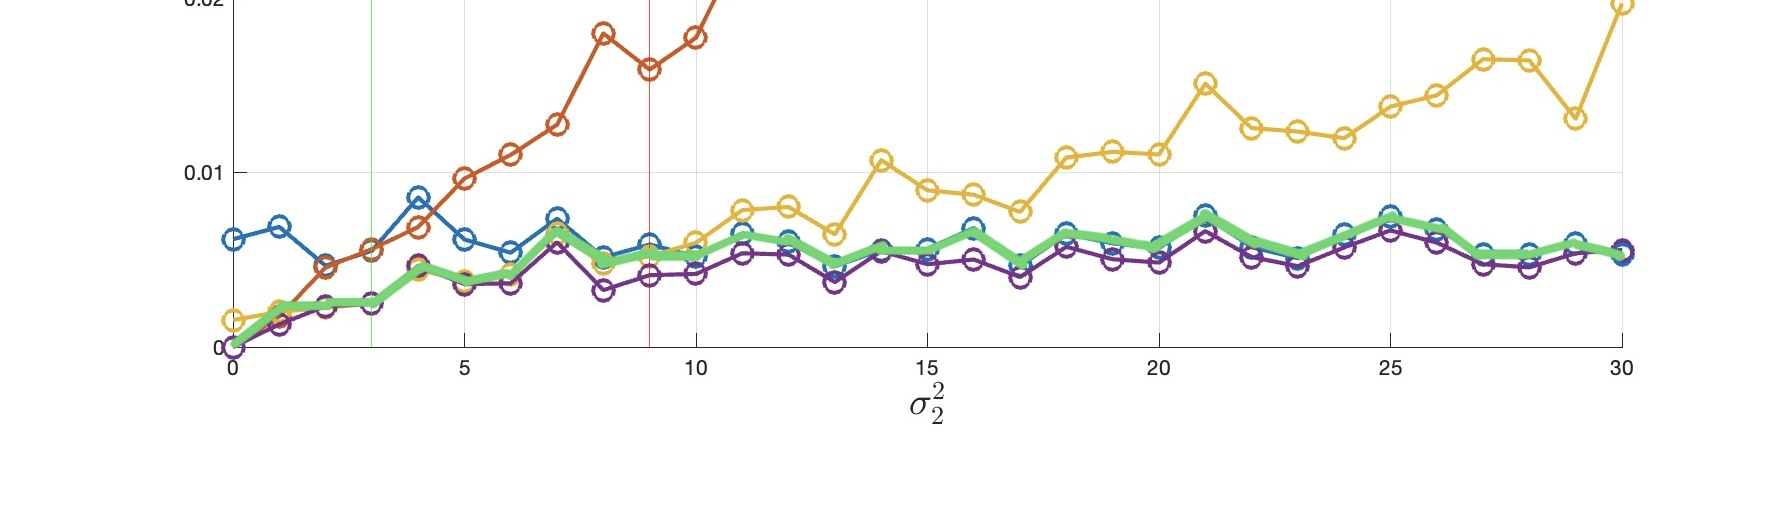
\includegraphics[width=\textwidth]{./figures/appendix_a/figure_2.jpeg}
\end{figure}

Let us observe the comparison between the theoretical error (corresponding to the variance as we have previously said) and the estimated MSE.

\begin{figure}[H]
    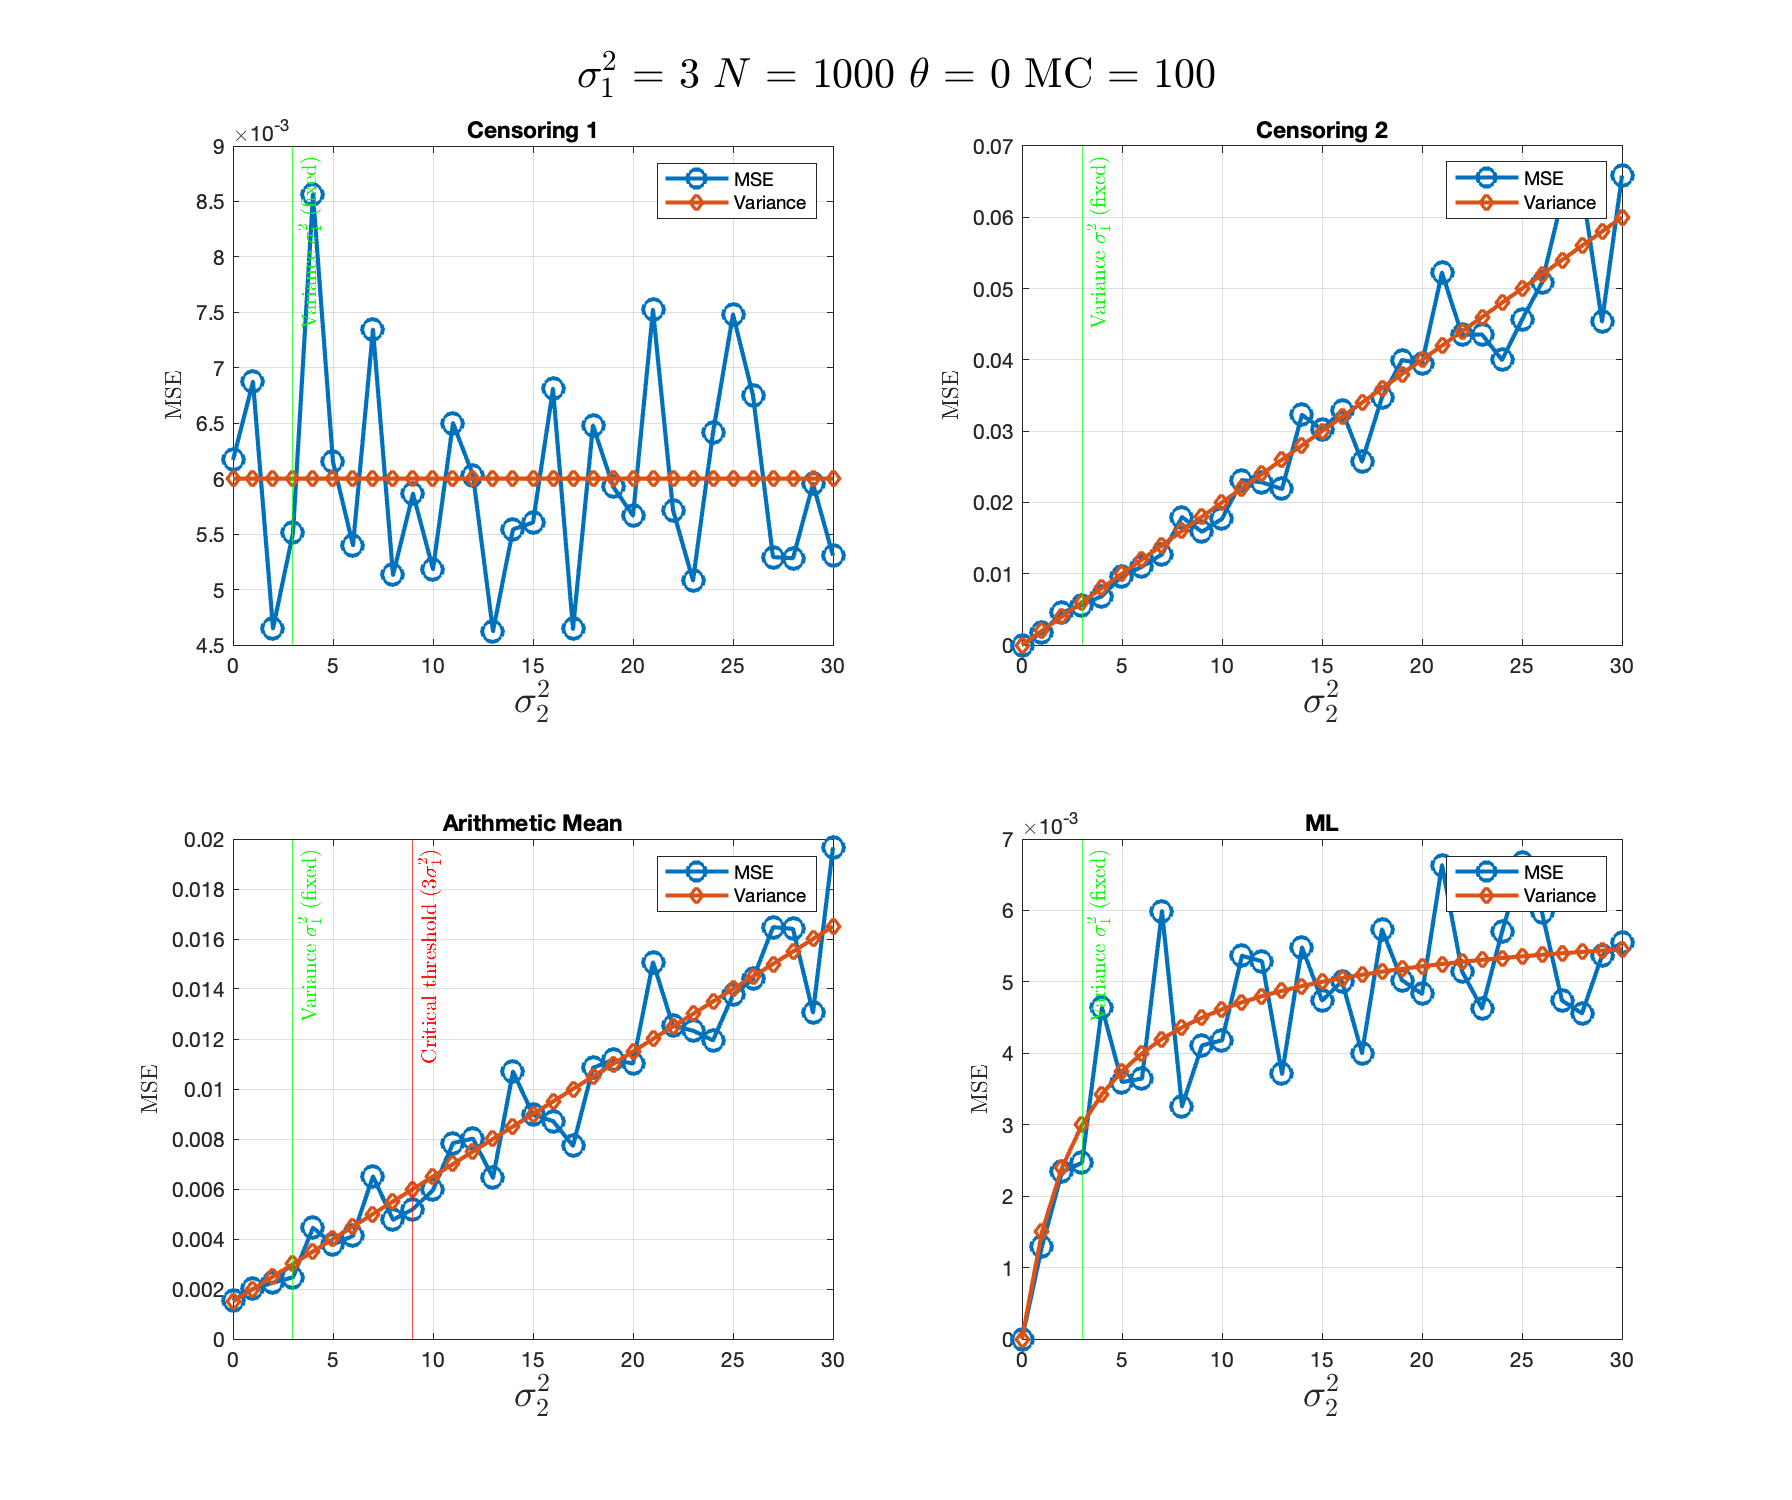
\includegraphics[width=\textwidth]{./figures/appendix_a/figure_3.png}
\end{figure}

\textit{If I have more noise the error is greater and in fact we have seen how increasing the variance increases the error in general. But if I want to estimate that error with the Monte Carlo simulation, with noisier data it is more complex to make the estimate?}

The answer is clearly yes, if I have noisier data everything seems more random and therefore I need more simulations. Let us observe what happens if we increase the number of simulations by an order of magnitude.

\begin{figure}[H]
    \centering
    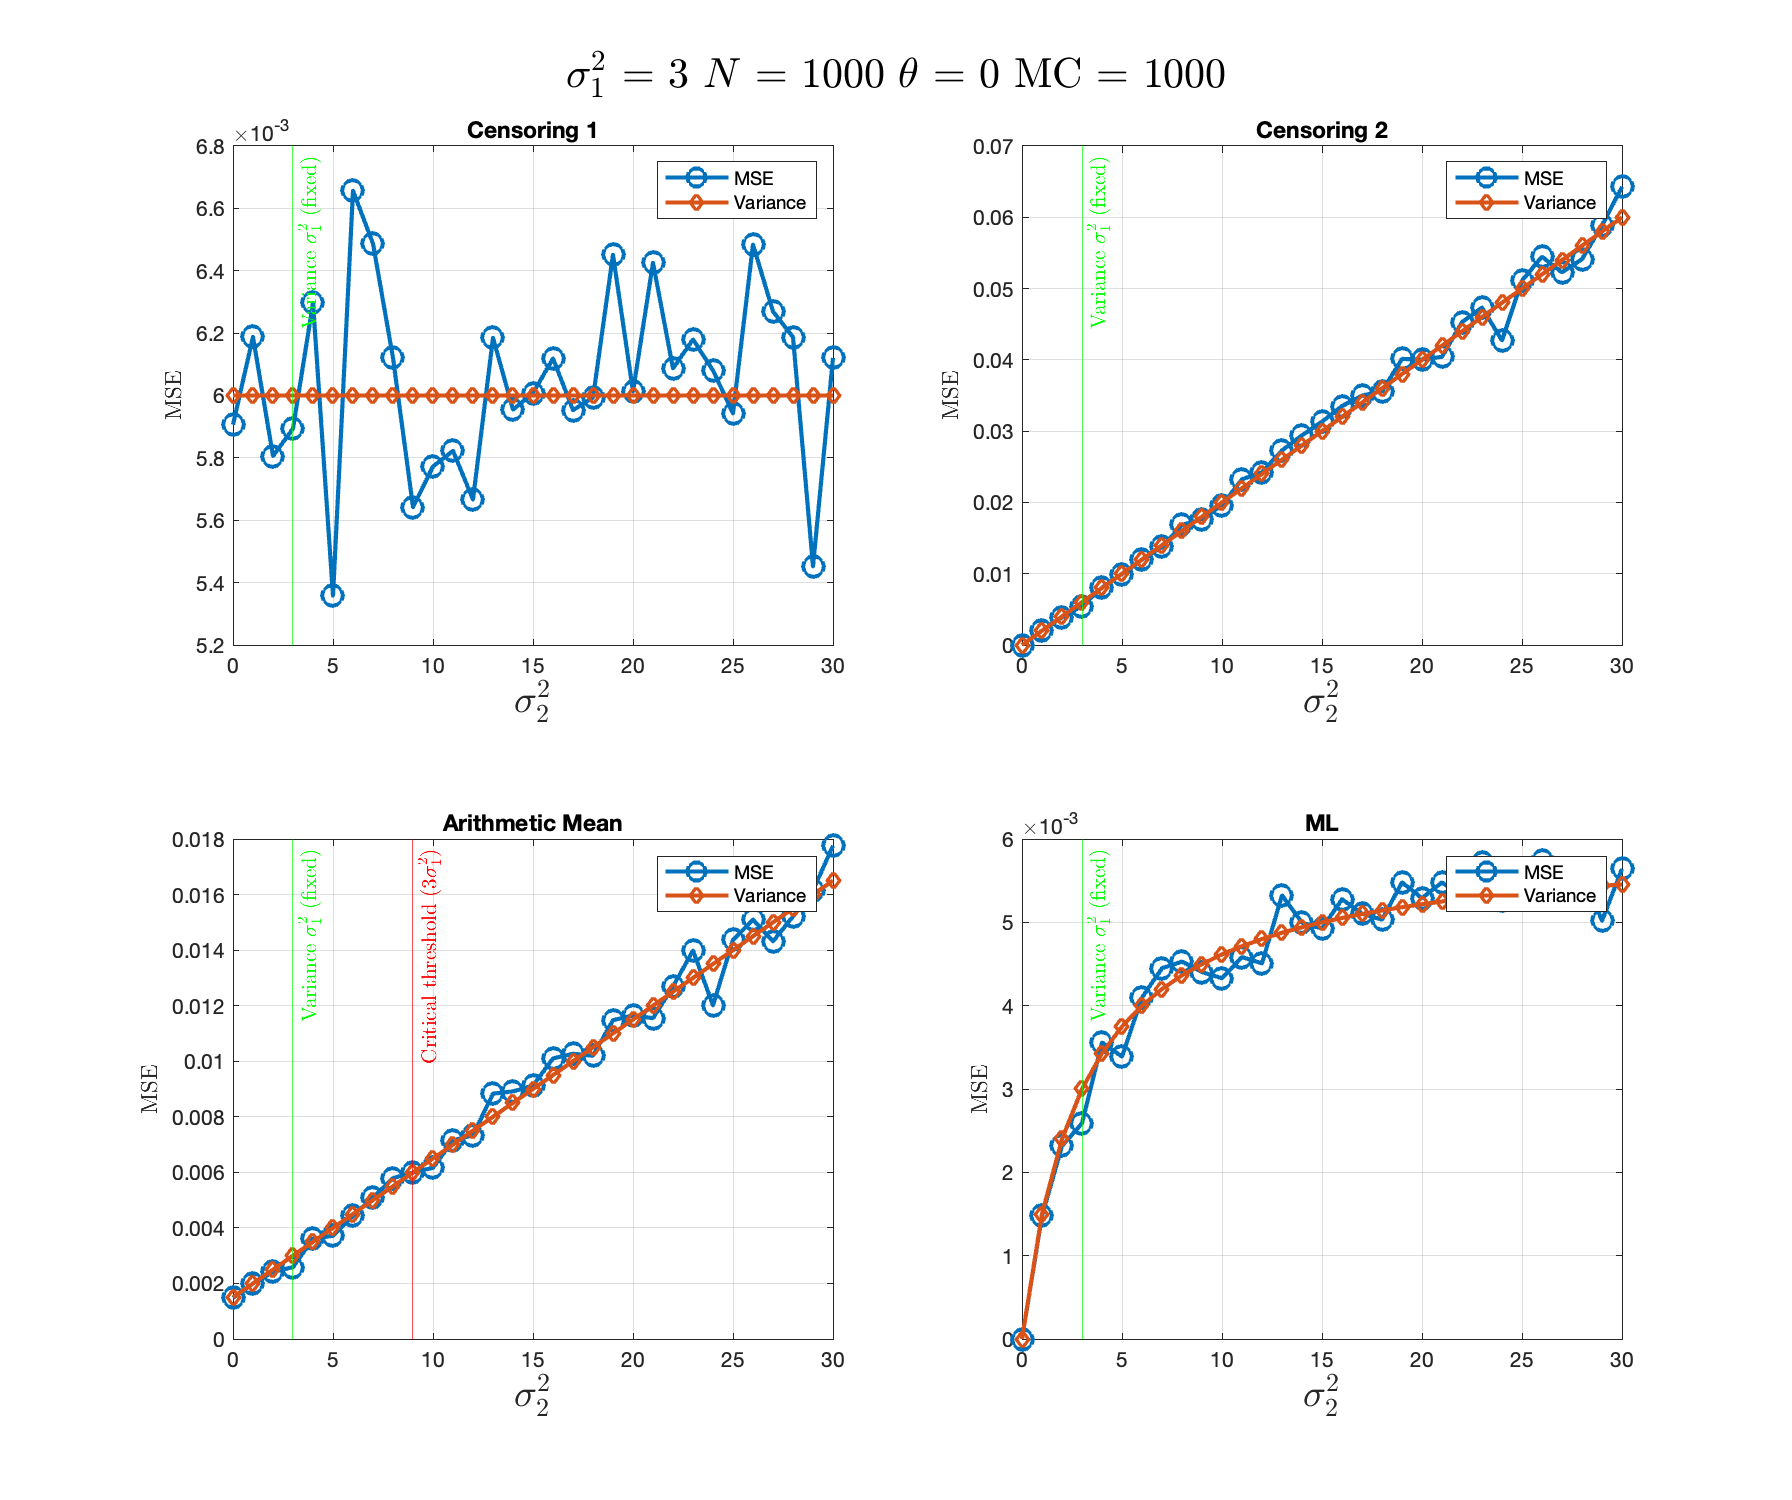
\includegraphics[width=\textwidth]{./figures/appendix_a/figure_4.png}
\end{figure}

\subsection*{Variation of $N$}

Let's look at the variation of the MSE as $N$ increases, both using a linear scale for the y-axis and a logarithmic scale. We also perform a comprehensive analysis from the perspective of the two scenarios we could encounter: $\sigma_2^2>3\sigma_1^2$ and $\sigma_2^2\le3\sigma_1^2$.

We can observe that using both logarithmic scales, the curve has a linear trend. This means that the actual trend is a power of $N$, specifically in this case $N^{-1}$. All these curves decrease with the same law (\textbf{scaling law}, often a theoretical result is expressed in terms of it). This is also derived from theory as the theoretical error decreases proportionally to $N$.

\begin{note}{About scaling laws}
A scaling law is 
$$
y=a\cdot x^b
$$

If we used a logarithmic scale to represent this relationship we would have:
$$
\log(y)=\log(a\cdot xb)=\log(a)+b\cdot\log(x)
$$

Since increasing $x$ the curve decreases with a unit slope, the value of $b=-1$, net of the proportionality coefficient $a$ which is different for all the curves.
\end{note}
\begin{note}{Comparison between scaling laws}
For this type of problems $\frac 1N$ is the best scaling law we could have in an independent sample estimation problem. So an estimator with this scaling law can be considered a good estimator, although the constant may then make the difference between estimators with the same scaling law.  
Only in extremely particular cases can we have exponential scaling laws.
\end{note}

The estimator $\hat\theta_{ML}$ not only has a scaling law of $\frac 1N$, but also has a smaller constant compared to the other estimators. In fact, we can observe that its curve is lower than the others.

We notice that in the two cases, respectively to the right and to the left of the threshold on the variance that emerged from the theory, we have a different ordering of the curves of $\hat\theta_{ave}$ and $\hat \theta_1$.


\section{MMSE}
% TODO: 
\section{Supervised Non Parametric Regression}
% TODO: 
\section{Classification}
% TODO: 